\documentclass[conference]{IEEEtran}
\IEEEoverridecommandlockouts
% The preceding line is only needed to identify funding in the first footnote. If that is unneeded, please comment it out.
\usepackage[hidelinks]{hyperref}
\urlstyle{same}
\usepackage[spanish,es-tabla]{babel}
\usepackage{cite}
\usepackage{amsmath,amssymb,amsfonts}
\usepackage{algorithmic}
\usepackage{graphicx}
\usepackage{textcomp}
\usepackage{xcolor}
\decimalpoint
\renewcommand{\labelitemi}{$\bullet$}
\def\BibTeX{{\rm B\kern-.05em{\sc i\kern-.025em b}\kern-.08em
    T\kern-.1667em\lower.7ex\hbox{E}\kern-.125emX}}
    
    
 %-------------------------------------------------------------------------------
%                            Libreria de codigos                               %
%-------------------------------------------------------------------------------
% Paquetes necesarios
\usepackage{listings}
\usepackage{xcolor}
\usepackage{comment}

% Tipos de letra personalizadas
\def\lstbasicfont{\fontfamily{pcr}\selectfont\scriptsize}
\def\vhdlbasicfont{\fontfamily{cmtt}\selectfont\scriptsize}

% Colores personalizados
\definecolor{codegreen}{rgb}{0,0.6,0}
\definecolor{codepurple}{rgb}{0.58,0,0.82}

\definecolor{codegray}{rgb}{0.5,0.5,0.5}
\definecolor{backcolour}{rgb}{0.95,0.95,0.92}
\definecolor{codeorange}{RGB}{254, 100, 35}

% Deficion de lenguajes perzonalizados

% Definicion de lenguaje MATLAB
\lstdefinelanguage{matlabfloz}{%
  alsoletter={...},%
  morekeywords={%                             % keywords
		break,case,catch,classdef,continue,else,
		elseif,end,for,function,global,if,
		otherwise,parfor,persistent,
		return,spmd,switch,try,while,...},        % Use the matlab "iskeyword" command to get those
  comment=[l]\%,                              % comments
  morecomment=[l]...,                         % comments
  morecomment=[s]{\%\{}{\%\}},                % block comments
  morestring=[m]'                             % strings 
}[keywords,comments,strings]%

% Estilos MATLAB
\lstdefinestyle{MATLAB}{
	frame=single,
	rulecolor=\color{black},
	framexleftmargin=4mm,
	xleftmargin=2mm,
	language=matlabfloz,
  commentstyle=\color{codegreen},
  keywordstyle=\color{blue}, %magenta
  numberstyle=\tiny\color{black},
  stringstyle=\color{codepurple},
  basicstyle=\lstbasicfont\scriptsize,
  breakatwhitespace=false,         
  breaklines=true,                 
  captionpos=b,                    
  keepspaces=true,                 
  numbers=left,                    
  numbersep=5pt,                  
  showspaces=false,                
  showstringspaces=false,
  showtabs=false,                  
  tabsize=2    
}

\lstdefinestyle{PYTHON}{
	frame=single,
	rulecolor=\color{black},
	framexleftmargin=4mm,
	xleftmargin=2mm,
	language=python,
    backgroundcolor=\color{backcolour},   
    commentstyle=\color{codegreen},
    keywordstyle=\color{blue}, %magenta
    numberstyle=\tiny\color{black},
    stringstyle=\color{codeorange},
    basicstyle=\lstbasicfont\footnotesize,
    breakatwhitespace=false,         
    breaklines=true,                 
    captionpos=b,                    
    keepspaces=true,                 
    numbers=left,                    
    numbersep=5pt,                  
    showspaces=false,                
    showstringspaces=false,
    showtabs=false,                  
    tabsize=2,
    otherkeywords = {show,arange}  
}



\lstdefinestyle{BASH}{
	frame=single,
	rulecolor=\color{black},
	framexleftmargin=4mm,
	xleftmargin=2mm,
	language=bash,
    %backgroundcolor=\color{backcolour},   
    commentstyle=\color{codegreen},
    keywordstyle=\color{blue}, %magenta
    numberstyle=\tiny\color{black},
    stringstyle=\color{codeorange},
    basicstyle=\lstbasicfont\footnotesize,
    breakatwhitespace=false,         
    breaklines=true,                 
    captionpos=b,                    
    keepspaces=true,                 
    numbers=left,                    
    numbersep=5pt,                  
    showspaces=false,                
    showstringspaces=false,
    showtabs=false,                  
    tabsize=2,
    %otherkeywords = {show,arange}  
}

\renewcommand{\lstlistingname}{Código}% Listing -> Algorithm
\renewcommand{\lstlistlistingname}{Lista de códigos}% 
\begin{document}

\title{Tarea 5: Optimización multiobjetivo utilizando el algoritmo de MOEAD y MOMBI2 para resolver el problema de Tanaka
}

\author{\IEEEauthorblockN{Ciro Fabian Bermudez Marquez}
INAOE\\
Mexico, Puebla \\
\url{cirofabian.bermudez@gmail.com}
}

\maketitle

\begin{abstract}
En este trabajo se ponen a prueba los algoritmos MOEAD y MOMBI2I para resolver el problema de  Tanaka.
\end{abstract}



\section{Descripción del problema}

Utilizando los algoritmos de MOEAD y MOMBI2 resolver el problema de Tanaka el cual esta codificado en lenguaje C y se presenta en la siguiente sección.


\section{Problema de Tanaka (1995)}
El problema de Tamaka es un problema de dos variables, dos objetivos y dos restricciones definido de la siguiente manera:

Minimizar:
\begin{equation}
f_{1}(\mathbf{x}) = x_{1} \qquad f_{2}(\mathbf{x}) = x_{2}
\end{equation}

Sujeto a:
\begin{equation}
C_{1}(\mathbf{x})  = x_{1}^{2} + x_{2}^{2} - 1 - 0.1 \cos \left(  16 \arctan \frac{x_{1}}{x_{2}}\right) \geq 0  
\end{equation}

\begin{equation}
C_{2}(\mathbf{x})  = (x_{1} -0.5)^{2} + (x_{2} -0.5)^{2}  \leq 0.5 
\end{equation}

\begin{equation}
0 \leq x_{1} \leq \pi \qquad 0 \leq x_{2} \leq \pi
\end{equation}

donde $\mathbf{x} = \left[ x_{1}, x_{2} \right]^{T}$.

\section{Resultados}

\section{MOEAD}

En las Figuras \ref{fig:tanaka1}, \ref{fig:tanaka2}, \ref{fig:tanaka3} se muestra el frente de Pareto al ejecutar en tres ocasiones el algoritmo de MOEAD:
\begin{figure}[hbtp]
\centering
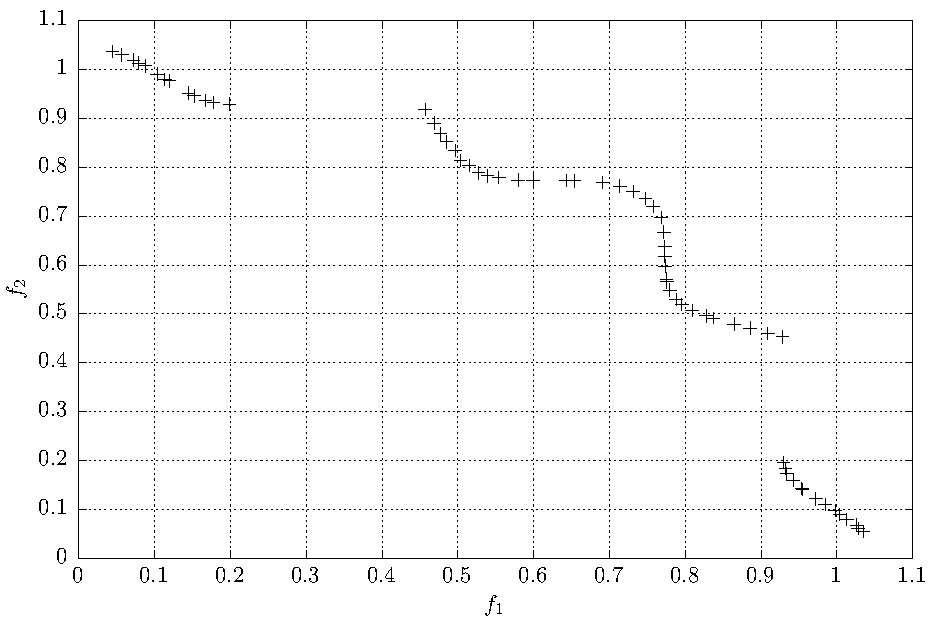
\includegraphics[width=7cm]{MOE1.pdf}
\caption{Frente de Pareto para el problema de Tanaka 1}
\label{fig:tanaka1}
\end{figure}

\begin{figure}[hbtp]
\centering
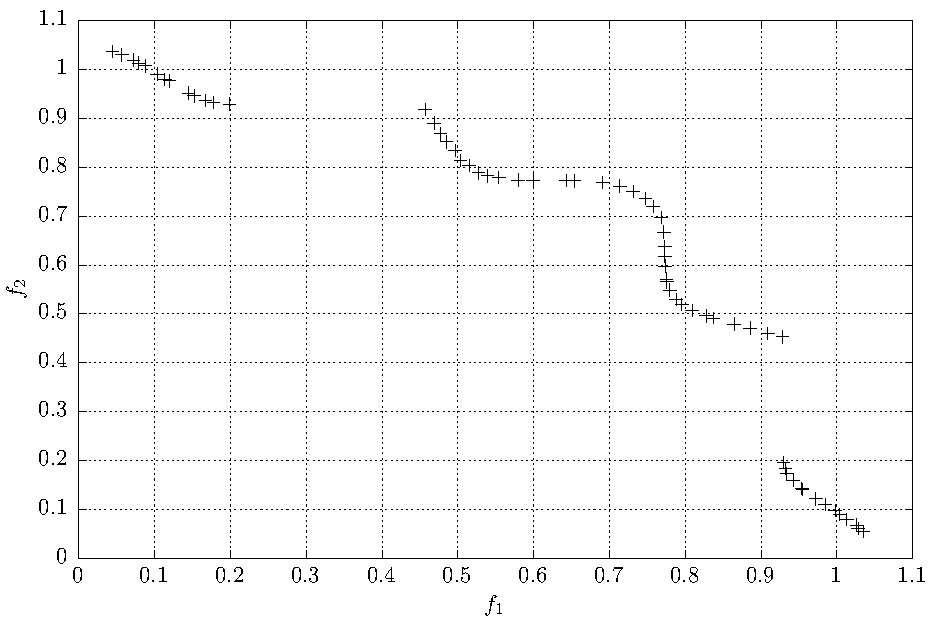
\includegraphics[width=7cm]{MOE2.pdf}
\caption{Frente de Pareto para el problema de Tanaka  2.}
\label{fig:tanaka2}
\end{figure}

\begin{figure}[hbtp]
\centering
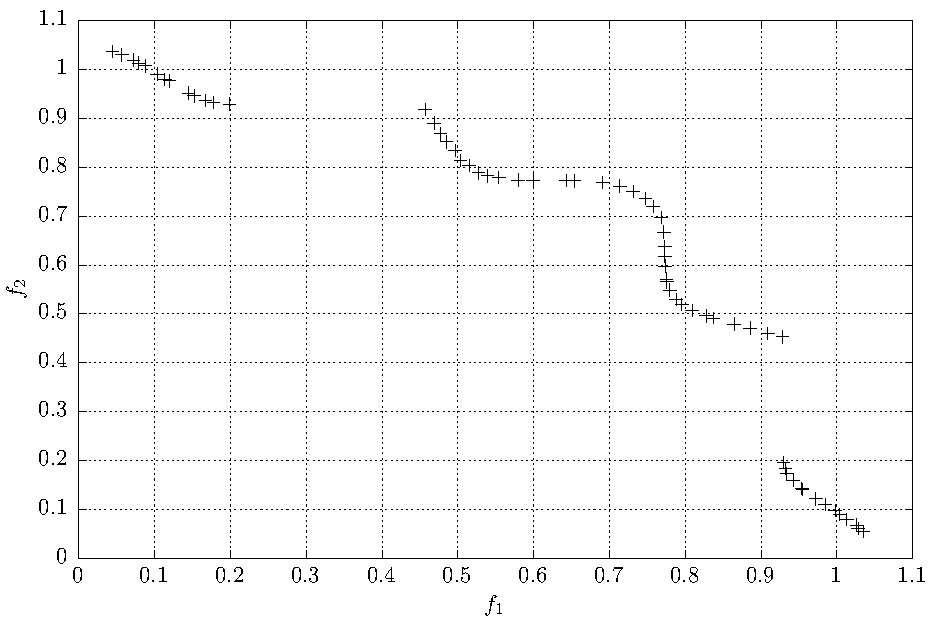
\includegraphics[width=7cm]{MOE3.pdf}
\caption{Frente de Pareto para el problema de Tanaka 3.}
\label{fig:tanaka3}
\end{figure}

\section{MOMBI2}
En las Figuras \ref{fig:1tanaka1}, \ref{fig:1tanaka2}, \ref{fig:1tanaka3} se muestra el frente de Pareto al ejecutar en tres ocasiones el algoritmo de MOEAD:
\begin{figure}[hbtp]
\centering
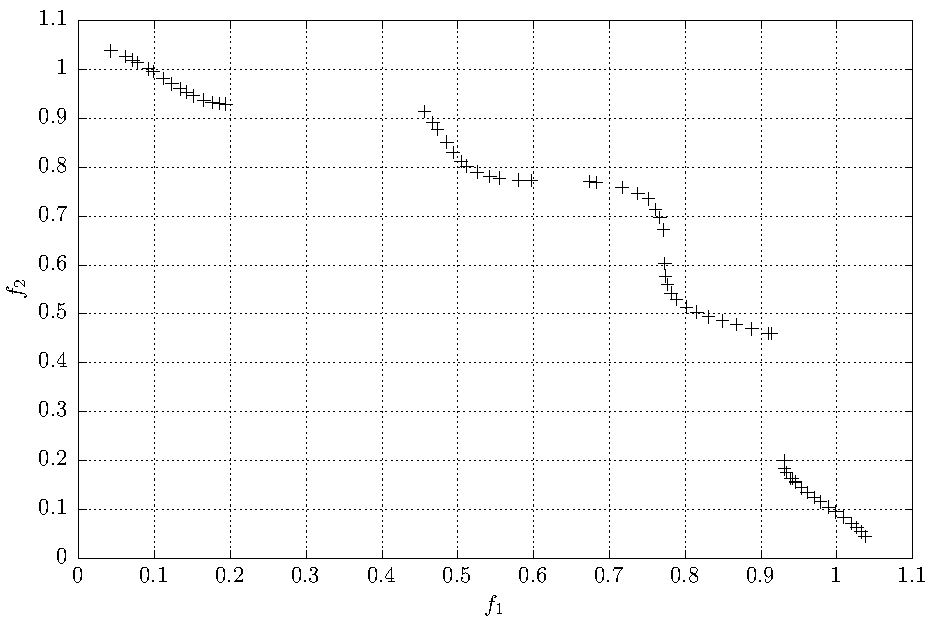
\includegraphics[width=7cm]{MOM1.pdf}
\caption{Frente de Pareto para el problema de Tanaka 1}
\label{fig:1tanaka1}
\end{figure}

\begin{figure}[hbtp]
\centering
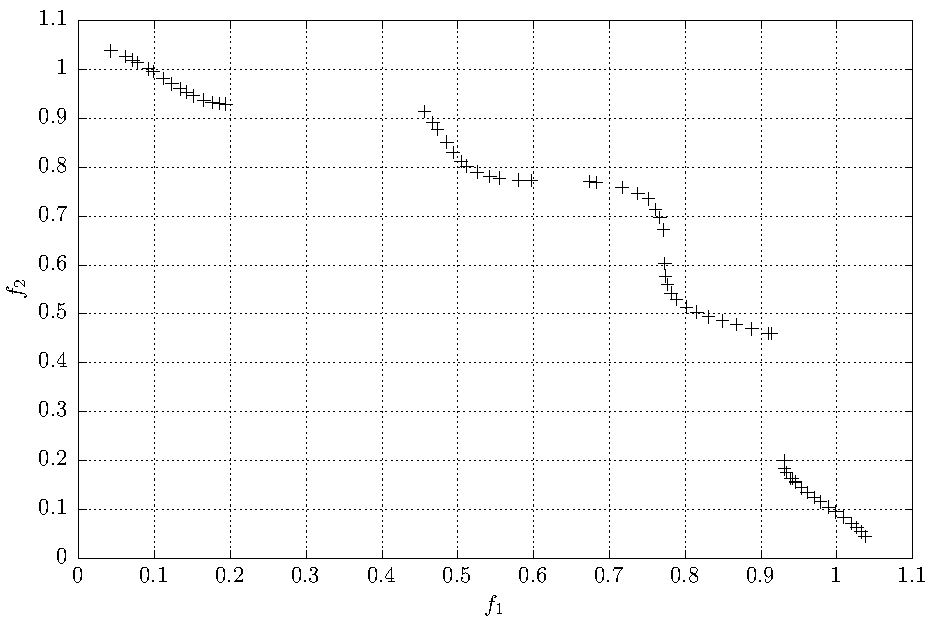
\includegraphics[width=7cm]{MOM2.pdf}
\caption{Frente de Pareto para el problema de Tanaka  2.}
\label{fig:1tanaka2}
\end{figure}

\begin{figure}[hbtp]
\centering
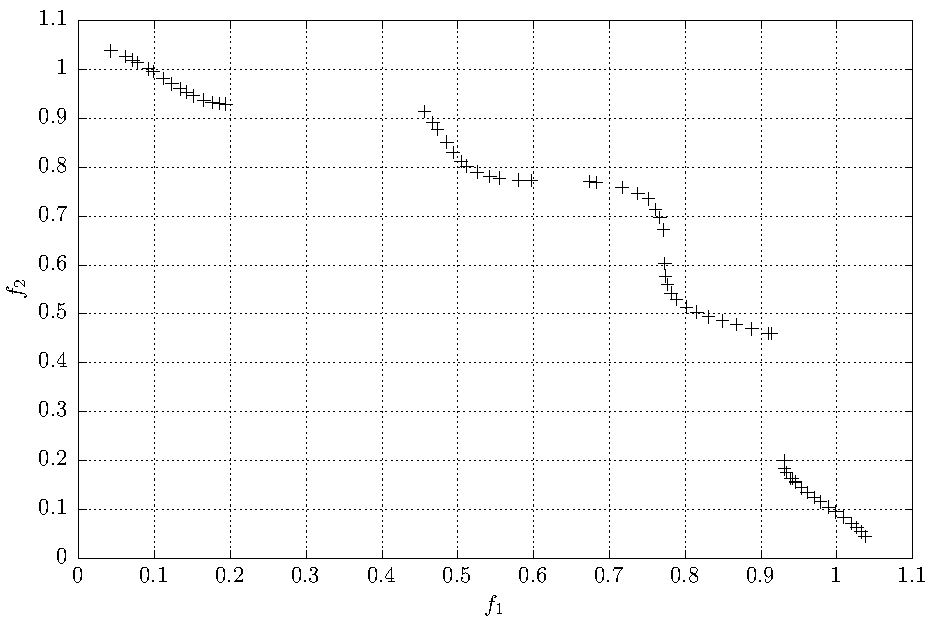
\includegraphics[width=7cm]{MOM3.pdf}
\caption{Frente de Pareto para el problema de Tanaka 3.}
\label{fig:1tanaka3}
\end{figure}

\section{Conclusiones}

El código de EMO Project es una herramienta en muy práctica que contiene muchos algoritmos para resolver problemas multiobjetivo, es este trabajo se probaron dos algoritmos MOEAD y MOMBI2, de los cuales se obtuvieron resultados muy parecidos. cabe resaltar que el tiempo de ejecución en ambos fue muy corto debido a su codificación en C y que los frentes de Pareto coinciden en su totalidad con los reportados por la literatura \cite{b2}.


\begin{thebibliography}{00}
\bibitem{b1}  Dr. Luis Gerardo de la Fraga. ``Apuntes de clase'' .
\bibitem{b2} Kalyanmoy Deb.``Multi-objetive Optimization using Evolutionary Algoritms'', John Wiley, 1ra Ed.
\end{thebibliography}


\end{document}
